\section{Introduction}

\subsection{Project Background}
The development of RAVEN started in 2012 when, within the Nuclear Energy
Advanced Modeling and Simulation (NEAMS) program~\cite{neams}, the need of a modern
risk evaluation framework arose.
RAVEN's principal assignment is to provide the necessary software and algorithms
in order to employ the concepts developed by the Risk Informed Safety Margin
Characterization (RISMC) Pathway.
RISMC is one of the pathways defined within the Light Water Reactor
Sustainability (LWRS) program~\cite{lwrs}.

The goal of the RISMC approach is  the identification not only of the frequency of an
event which can potentially lead to system failure, but also the proximity (or lack
thereof) to key safety-related events: the safety margin.
Hence, the approach is interested in identifying and increasing the safety
margins related to those events.
A safety margin is a numerical value quantifying the probability that a safety
metric (e.g. peak pressure in a pipe) is exceeded under certain conditions.
% Conclusion
Most of the capabilities, implemented having Reactor Excursion and Leak Analysis Program v.7
(RELAP-7) as a principal focus, are
easily deployable to other system codes.
%
For this reason, several side activates have been employed (e.g.  RELAP5-3D~\cite{RELAP5userManual}, any Multiphysics Object Oriented
Simulation Environment-based App, etc.)
or are currently ongoing for coupling RAVEN with several different software.
%

\subsection{Capabilities of RAVEN}
% High-level RAVEN description
RAVEN~\cite{alfonsiMC} ~\cite{alfonsiPSA}~\cite{RAVENFY13}~\cite{ESREL2014} is a software framework that allows the user to perform parametric and stochastic
analysis based on the response of complex system codes.
The initial development was designed to provide dynamic probabilistic risk analysis
capabilities (DPRA) to the thermal-hydraulic code RELAP-7~\cite{relap7FY12}, currently under development
at Idaho National Laboratory (INL).
Now, RAVEN is not only a framework to perform DPRA but it is a flexible and
multi-purpose uncertainty quantification, regression analysis, probabilistic risk assessment, data analysis and
model optimization platform. Depending on the tasks to be accomplished and on the probabilistic characterization
of the problem, RAVEN perturbs (e.g., Monte-Carlo, latin hypercube, reliability surface search) the response of
the system under consideration by altering its own parameters. The system is modeled by third party software
(e.g., RELAP5-3D, MAAP5, BISON, etc.) and accessible to RAVEN either directly (software coupling) or indirectly
(via input/output files). The data generated by the sampling process is analyzed using classical statistical
and more advanced data mining approaches. RAVEN also manages the parallel dispatching
(i.e. both on desktop/workstation and large High Performance Computing machines) of the software representing the
physical model. RAVEN heavily relies on artificial intelligence algorithms to construct surrogate models of
complex physical systems in order to perform uncertainty quantification, reliability analysis (limit state surface)
and parametric studies.

The main capabilities of RAVEN, with brief descriptions, are summarized here, or one can check the Figure.~\ref{fig:ravenCap}.
These capabilities may be used on their own or as building blocks to construct the sought workflow. In addition, RAVEN also provides some more sophisticated
\textbf{Ensemble algorithms} such as \textbf{EnsembleForward}, \textbf{EnsembleModel} to combine the existing
capabilites.

\begin{itemize}
  \item \textbf{Sensitivity Analysis and Uncertainty Quantification}: Sensitivity analysis is a mathematical tool
    that can be used to identify the key sources of uncertainties. Uncertainty quantification is a process by which
    probabilistic information about system responses can be computed according to specified input parameter probability
    distributions. Available approaches in RAVEN include \textbf{Monte Carlo}, \textbf{Grid}, \textbf{Stratified (Latin hypercube)},
    \textbf{Sparse Grid Collocation}, \textbf{Sobol}, \textbf{Adaptive Sparse Grid} and \textbf{Adaptive Sobol}.
  \item \textbf{Design of Experiments}: The design of experiments (DOE) is a powerful tool that can be used to explore the
    parameter space at a variety of experimental situations. It can be used to determine the relationship between
    input factors and the desired outputs. Available approaches in RAVEN include \textbf{Factorial Design}
    (i.e. General full factorial, 2-level fractional-factorial and Plackett-Burman) and \textbf{Response Surface Design}
    (i.e. Box-Behnken and Central composite algorithms).
  \item \textbf{Risk Mitigation or Model Optimization}: RAVEN uses the \textbf{Optimizer}, a powerful sampler-like entity that searches
    the input space to find minimum or maximum values of a reponse. Currently available optimizers include
    \textbf{Simultaneous Perturbation Stochastic Approximation (SPSA)}.
  \item \textbf{Risk Analysis}: Available approaches in RAVEN include \textbf{Dynamic Event Tree}, \textbf{Limit Surface Search},
    \textbf{Hybrid Dynamic Event Tree}, \textbf{Adaptive Dynamic Event Tree}, \textbf{Adaptive Hybrid Dynamic Event Tree},
    \textbf{Data Mining}, \textbf{Importance Rank}, \textbf{Safest Point}, and \textbf{Basic Statistics}.
  \item \textbf{Risk Management}: Available approaches in RAVEN include \textbf{Reduced order models},
    approaches used for sensitivity and uncertainty analysis, and \textbf{Dynamic Event Tree} methods.
  \item \textbf{Validation}: Available approaches in RAVEN include \textbf{ROMs}, \textbf{Comparison Statistics} and \textbf{Validation Metrics} 
\end{itemize}

In addition, RAVEN includes a number of related advanced capabilities. \textbf{Surrogate or Reduced order models (ROMs)} are mathematical
model trained to predict a response of interest of a physical system. Typically, ROMs trade speed for accuracy representing
a faster, rough estimate of the underlying systems. They can be used to explore the input parameter space for optimization
or sensitivity and uncertainty studies. \textbf{Ensemble Model} is able to combine \textbf{Codes}, \textbf{External Models}
and \textbf{ROMs}. It is aimed to create a chain of models whose execution order is determined by the input/output
relationships among them. If the relationships among the models evolve in a non-linear system, a Picard's iteration scheme is
employed.

\begin{figure}[h!]
  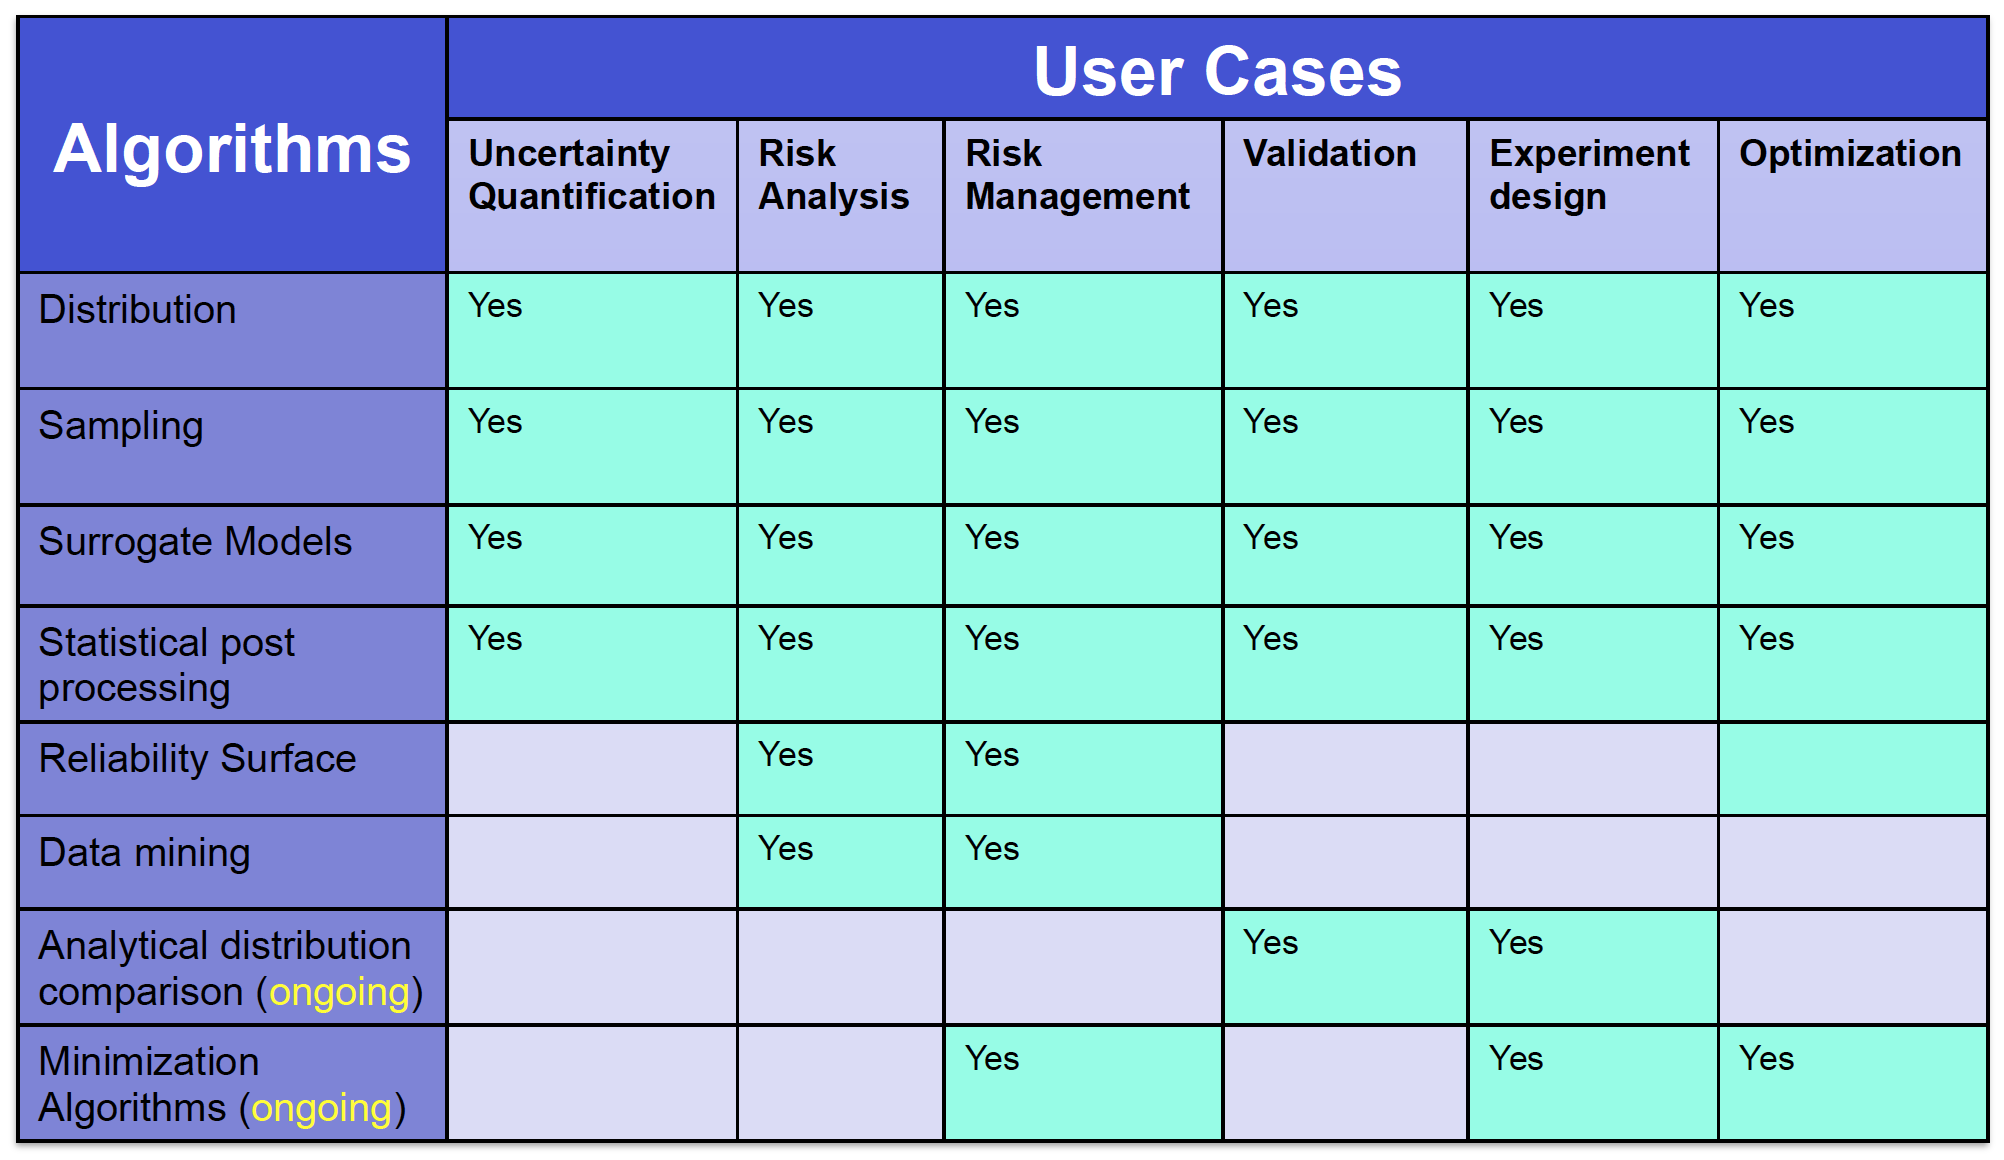
\includegraphics[width=\textwidth]{pics/raven_cap.png}
  \caption{RAVEN Capabilities vs. Needs}
  \label{fig:ravenCap}
\end{figure}

\subsection{Code Interfaces of RAVEN}
The procedure of coupling a new code/application with RAVEN is a straightforward process. The provided Application
Programming Interfaces (APIs) allow RAVEN to interact with any code as long as all the parameters that need to be
perturbed are accessible by input files or via python interfaces. For example, for all the codes currently
supported by RAVEN (e.g. RELAP-7, RELAP-5D, BISON, MAMMOTH, etc.), the coupling is performed through a Python interface
that interprets the information coming from RAVEN and translates them into the input of the driven code. The couping procedure
does not require modifying RAVEN itself. Instread, the developer creates a new Python interface that is going to
be embedded in RAVEN at run-time (no need to introduce hard-coded coupling statements). In addition, RAVEN will
manage concurrent executions of your simulations in parallel, whether on a local desktop or remote high-performance cluster.

Figure.~\ref{fig:modelAPIs} depicts the different APIs between RAVEN and the computational models, i.e. the
\textbf{ROM}, \textbf{External Models} and \textbf{External Code} APIs. 

\begin{figure}[h!]
  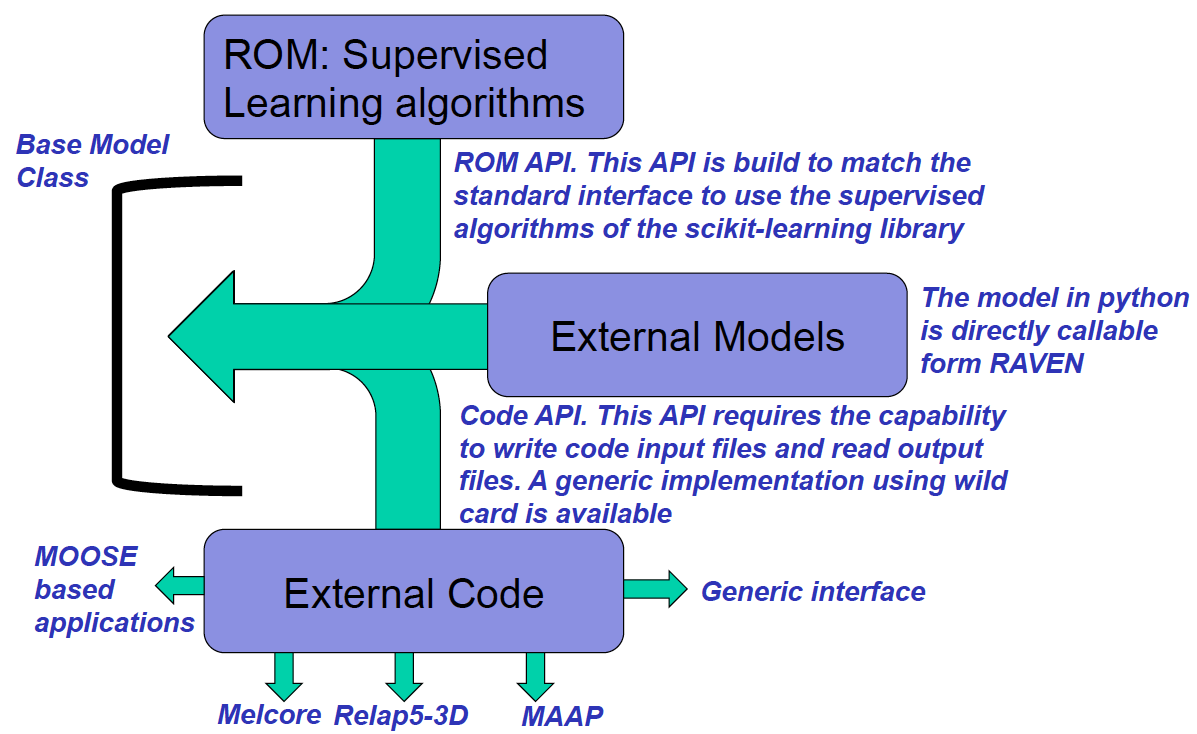
\includegraphics[width=\textwidth]{pics/modelAPIs.png}
  \caption{RAVEN Application Programming Interfaces}
  \label{fig:modelAPIs}
\end{figure}

\subsection{User Guide Organization}
The aim of this document is to provide a set of detailed examples that can help the user to become familiar with
the RAVEN code. RAVEN is capable of investigating system response and explore input space using various
sampling schemes such as Monte Carlo, grid, or Latin Hypercube. However, RAVEN strength lies in its system feature
discovery capabilities such as: constructing limit surfaces, separating regions of the input space leading to
system failure, and using dynamic supervised learning techniques. New users should consult the Tutorial to get started.
\begin{itemize}
  \item \textbf{RAVEN Tutorial}:
  \item \textbf{Sensitivity Analysis and Uncertainty Quantification}:
  \item \textbf{Model Optimization}:
  \item \textbf{Reduced Order Modeling}:
  \item \textbf{Data Mining}:
  \item \textbf{RAVEN Restart}:
  % Will be added latter
  %\item \textbf{Design of Experiments}:
  %\item \textbf{Risk Analysis}:
  %\item \textbf{Risk Management}:
  %\item \textbf{Validation}:
  %\item \textbf{Code Interface}:
  %\item \textbf{Advanced Topics}:
  %  \begin{itemize}
  %    \item Ensemble Forward Sampler:
  %    \item Ensemble Model:
  %  \end{itemize}
\end{itemize}



